\documentclass[svgnames,dvipsnames,hyperref={bookmarks=false},usepdftitle=false]{beamer}
\usetheme{scaladays}
\usepackage{tikz}
\usetikzlibrary[arrows.meta]

\title{Metaprogramming 2.0}
\author{Eugene Burmako (\href{https://twitter.com/xeno_by}{@xeno{\textunderscore}by})}
\institute{
\includegraphics[height=2cm]{epfl.png}}
\date{11 May 2016}
\hypersetup{pdfauthor={Eugene Burmako},pdftitle={Metaprogramming 2.0}}

\begin{document}

\titleframe

\begin{frame}{scala.meta is a dream}
\begin{center}
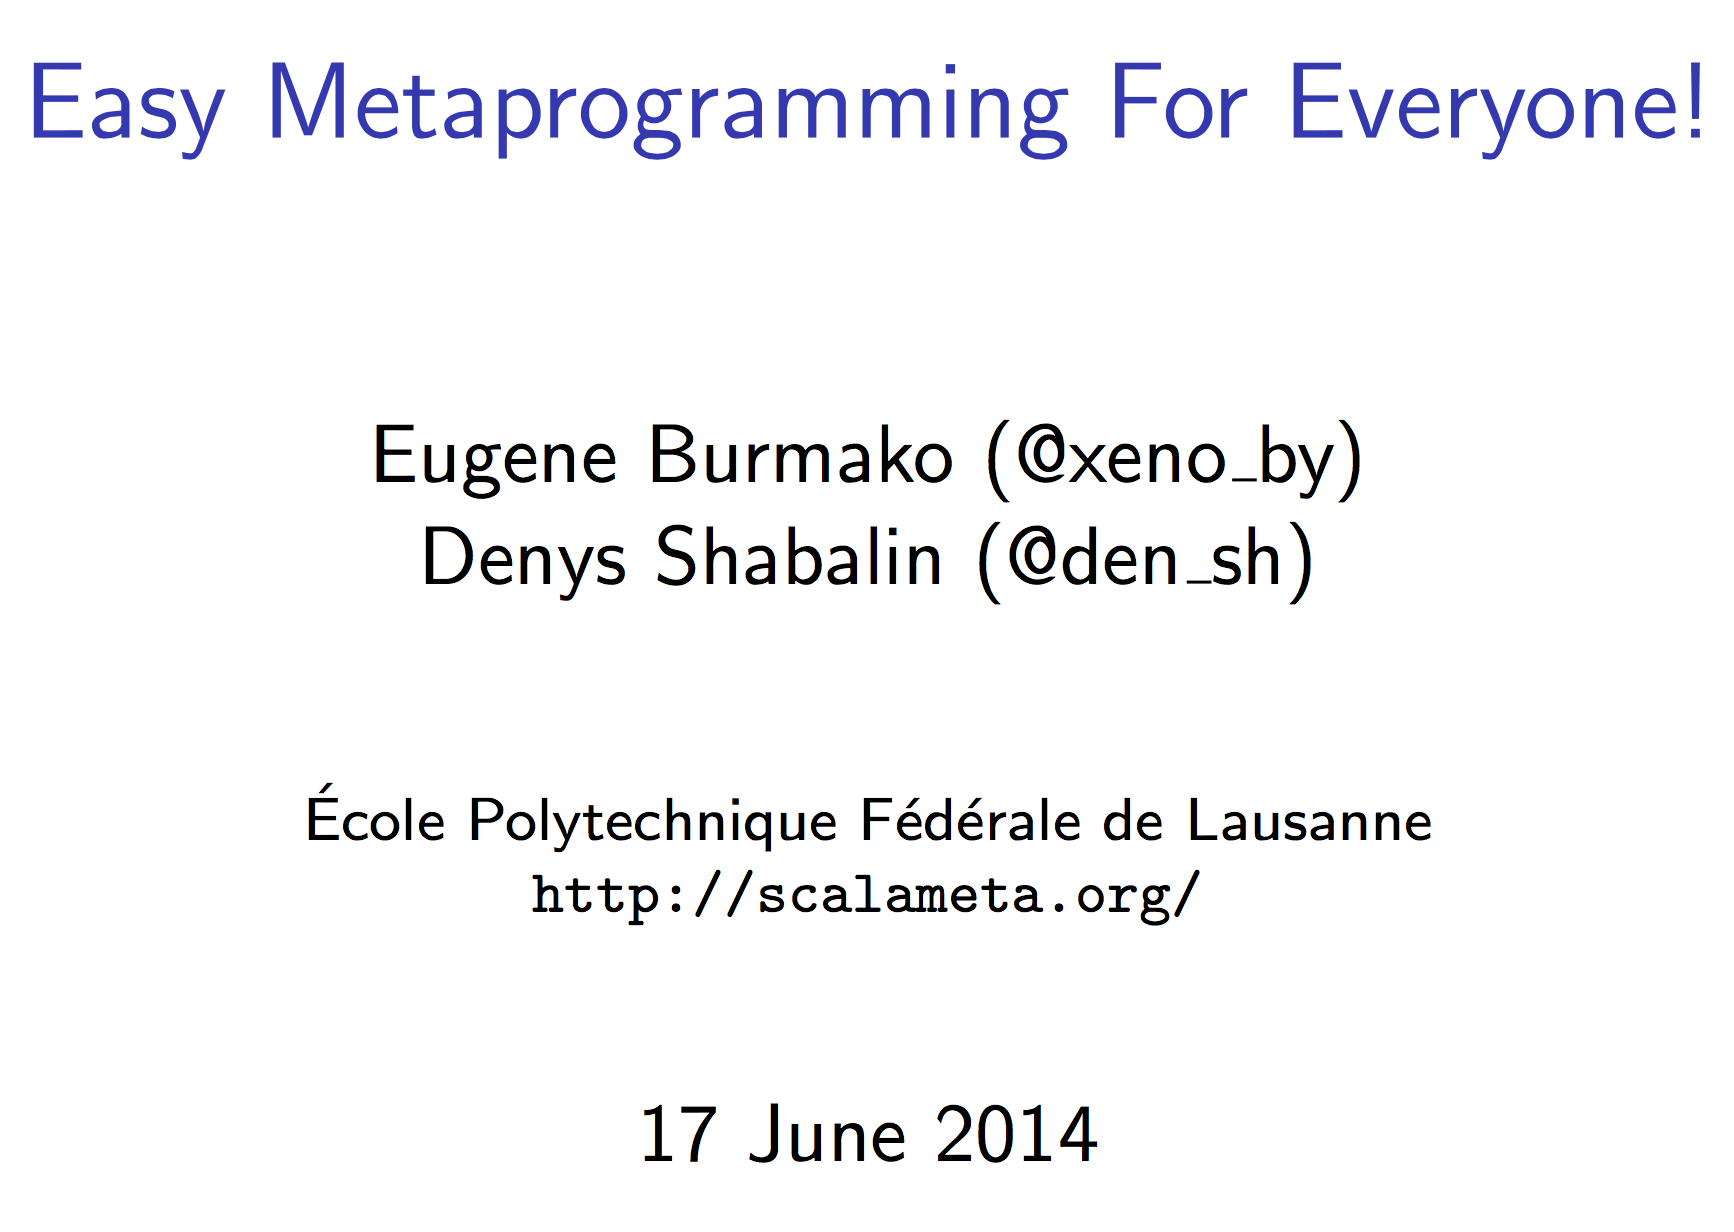
\includegraphics[height=6cm]{is-a-dream.png}
\end{center}
\end{frame}

\begin{frame}{scala.meta is an active project}
\vskip20pt
\begin{center}
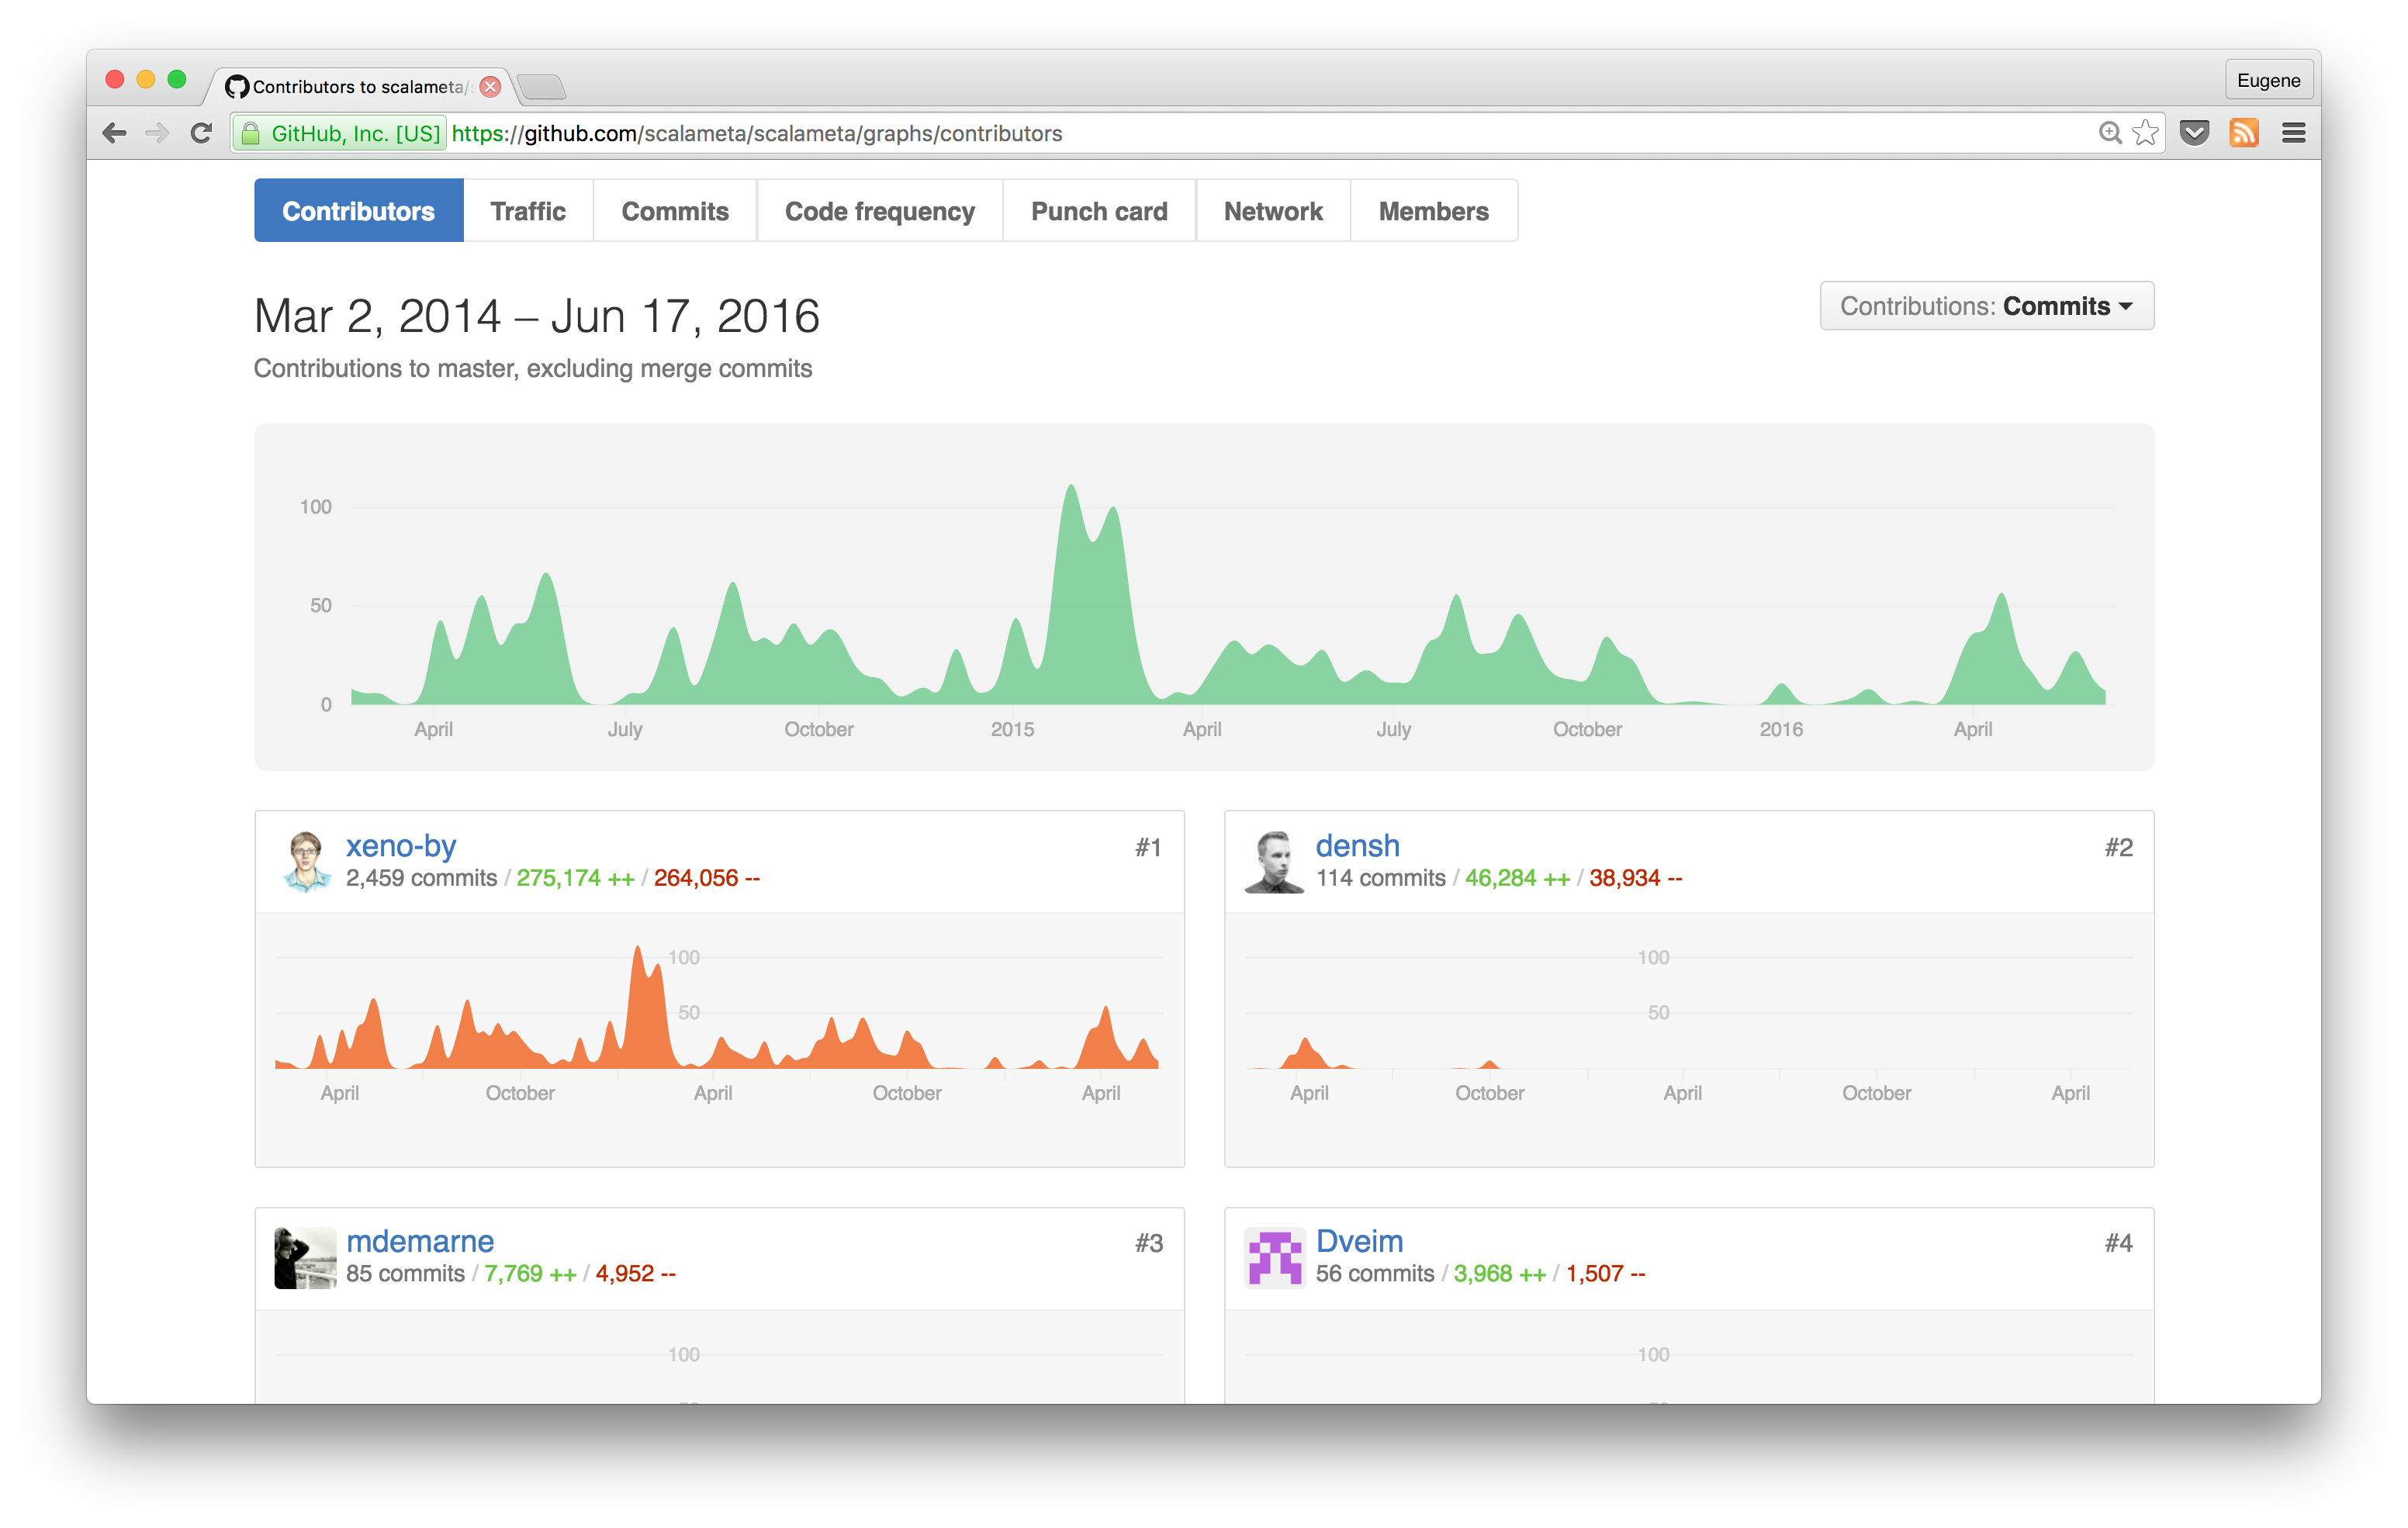
\includegraphics[height=7.5cm]{is-an-active-project.png}
\end{center}
\end{frame}

\begin{frame}{scala.meta is a community}
\vskip20pt
\begin{center}
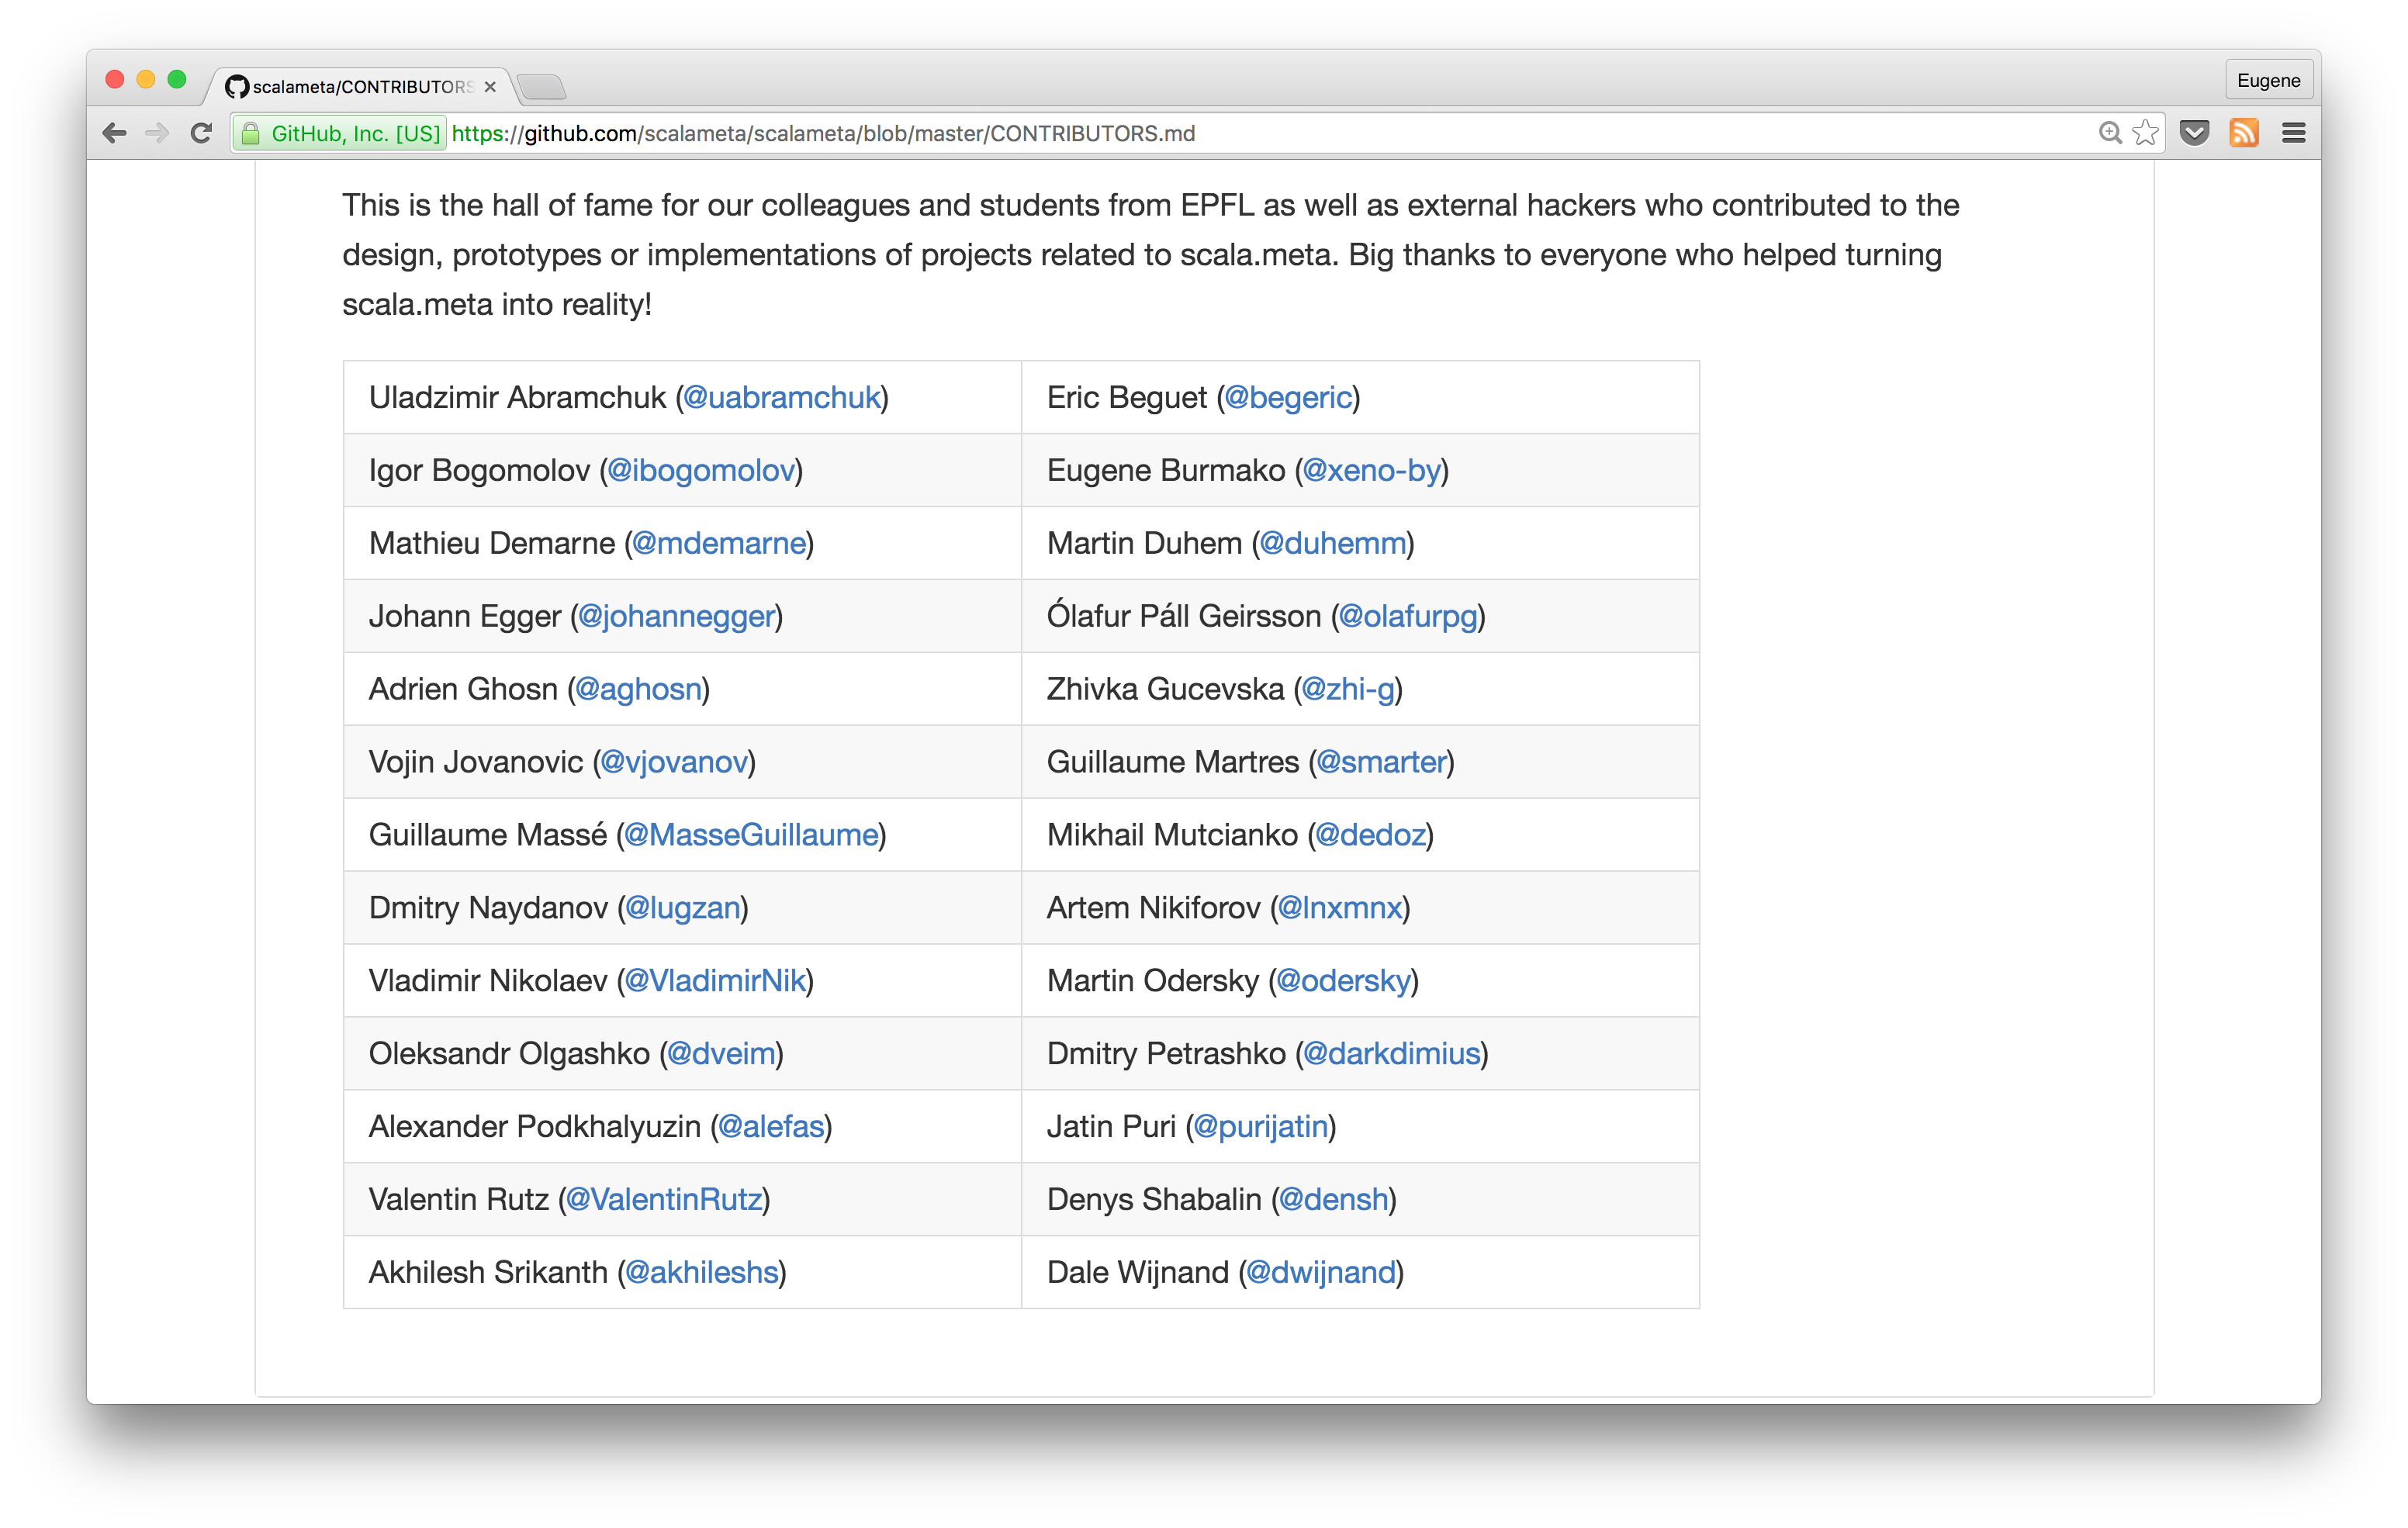
\includegraphics[height=7.5cm]{is-a-community.png}
\end{center}
\end{frame}

\begin{frame}{scala.meta is a product}
\vskip20pt
\begin{center}
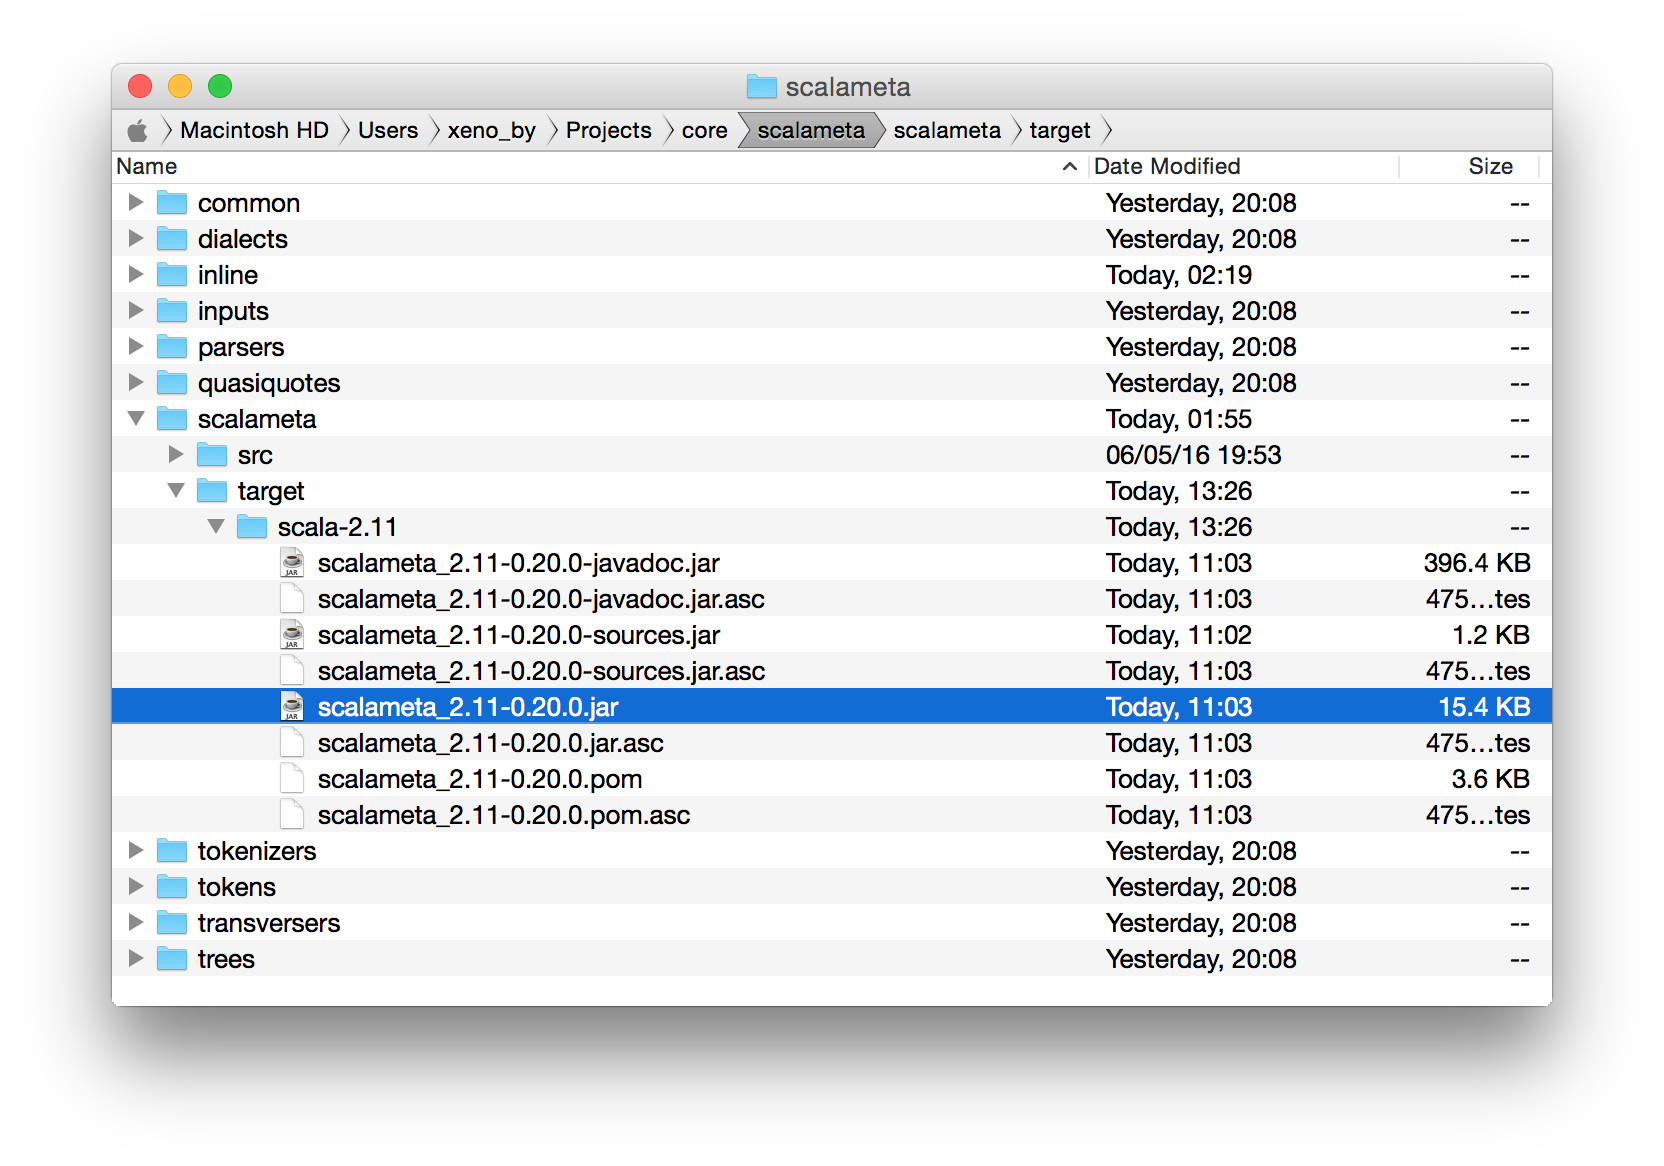
\includegraphics[height=8cm]{is-a-product.png}
\end{center}
\end{frame}

\begin{frame}{scala.meta is officially endorsed}
\vskip20pt
\begin{center}
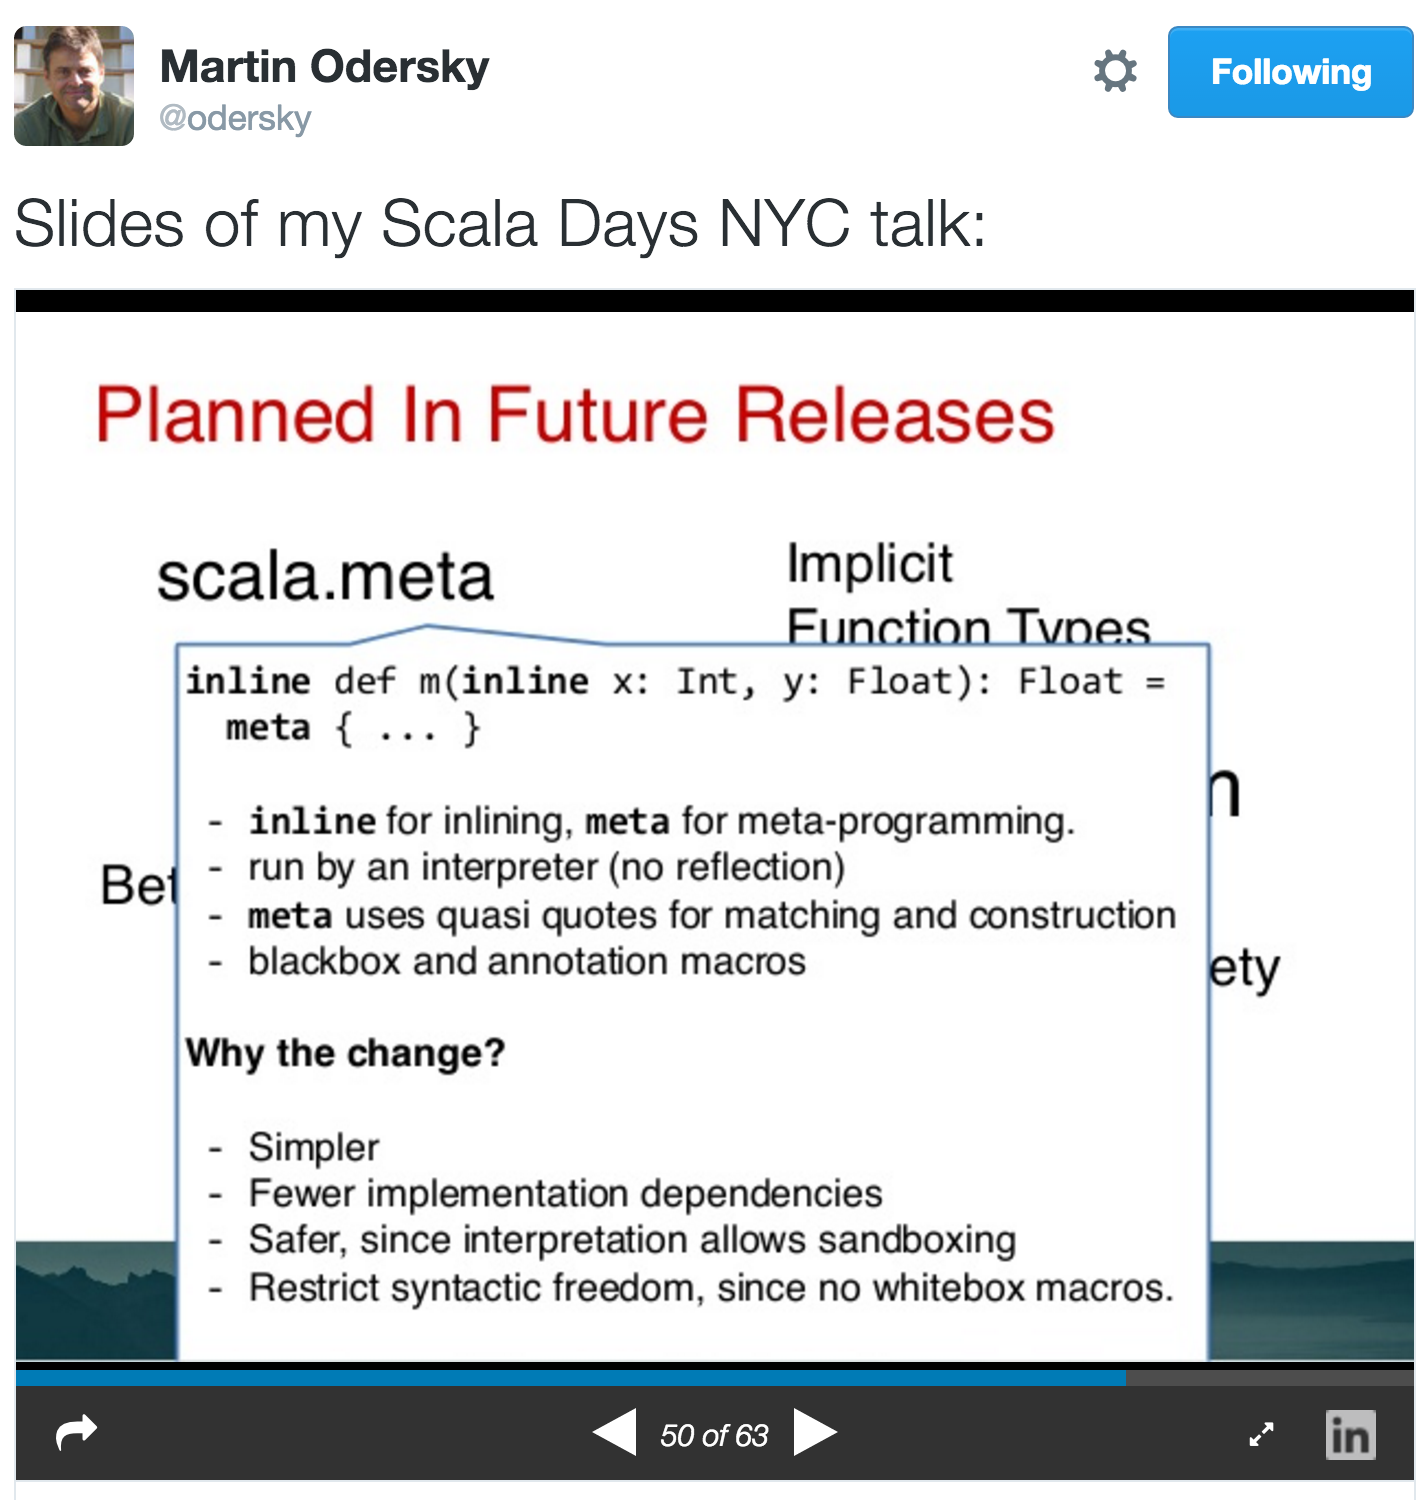
\includegraphics[height=7.5cm]{is-officially-endorsed.png}
\end{center}
\end{frame}

\sectionframe{Part 1: What can scala.meta do?}

\begin{frame}{ScalaDays 2015}
\begin{itemize}
\item Experimentation's temporarily on hold, we’re now pushing for 0.1
\item Main focus of 0.1 is making scala.meta trees publicly available
\end{itemize}
\end{frame}

\begin{frame}{ScalaDays 2016}
\begin{itemize}
\item 3k commits and 19 milestones later, we're almost there
\item Today we have published our first beta release: v0.20.0
\item We hope v1.0.0 to follow in the near future
\end{itemize}
\end{frame}

\begin{frame}{Supported functionality}
Feature-complete for v1.0.0:
\begin{itemize}
\item Parsing
\item Quasiquotes
\item Tokenization
\item Prettyprinting
\end{itemize}
\end{frame}

\begin{frame}{Future releases}
Planned for v2.0.0:
\begin{itemize}
\item AST persistence
\item Name resolution
\item Typechecking
\item Implicit inference
\end{itemize}
\end{frame}

\sectionframe{Part 2: Live demo}

\begin{frame}{Summary}
\begin{itemize}
\item Parsing different dialects of Scala
\item Type-safe quasiquotes
\item Tokenization for advanced tooling
\item Prettyprinting that respects formatting and comments
\end{itemize}
\end{frame}

\sectionframe{Part 3: But what about macros?}

\begin{frame}{}
\vskip20pt
\begin{center}

\includegraphics[height=7.5cm]{not-sure.jpg}
\end{center}
\end{frame}

\begin{frame}{Macros are dead}
\vskip20pt
\begin{center}
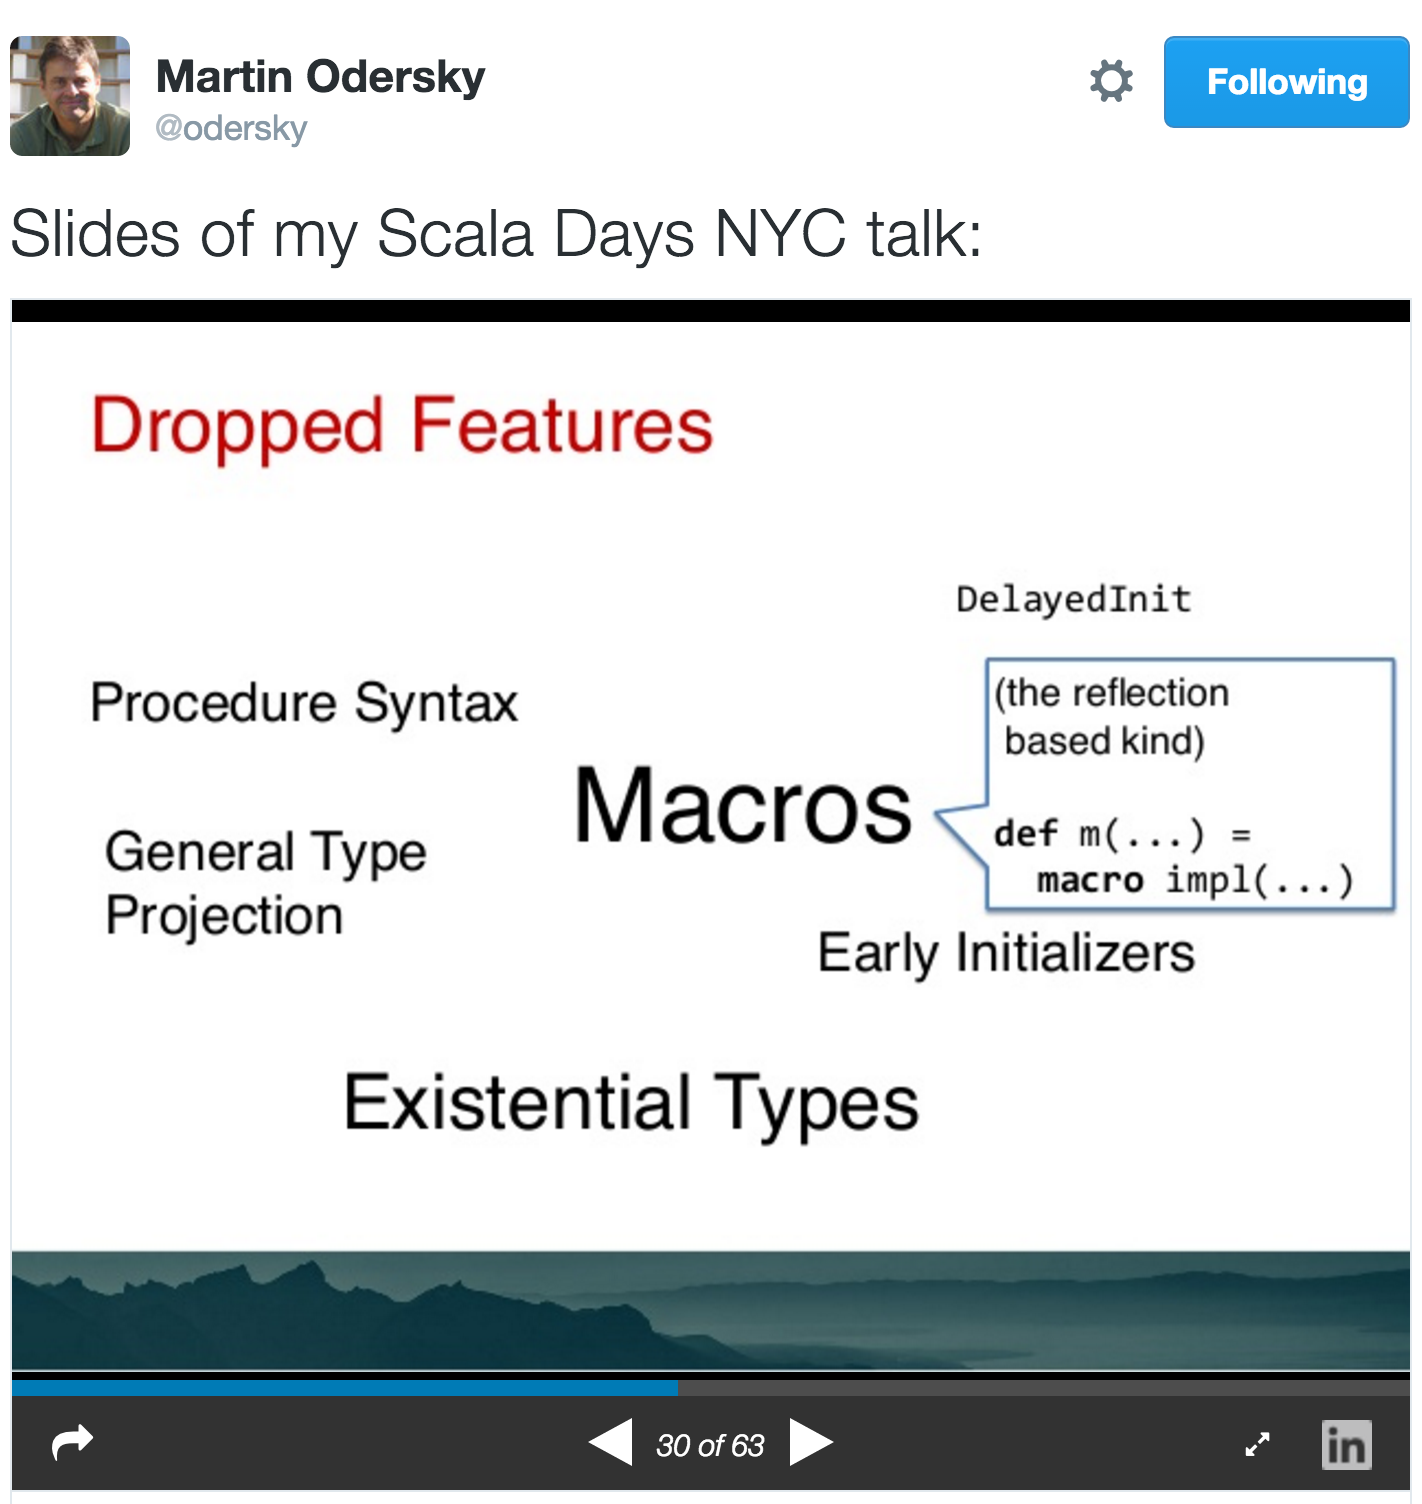
\includegraphics[height=7.5cm]{macros-are-dead.png}
\end{center}
\end{frame}

\begin{frame}{Macros are bad}
\begin{itemize}
\item Hard to write
\item Don't work with tools well
\item Hopelessly entangled with scalac
\end{itemize}
\end{frame}

\begin{frame}{Macros are great}
\begin{itemize}
\item Enable unique use cases
\item Frequently used by library authors
\item Most of the complexity is incidental
\end{itemize}
\end{frame}

\begin{frame}{Long live macros}
\vskip20pt
\begin{center}

\includegraphics[height=7.5cm]{long-live-macros.jpg}
\end{center}
\end{frame}

\begin{frame}{The new future for macros}
\vskip20pt
\begin{center}
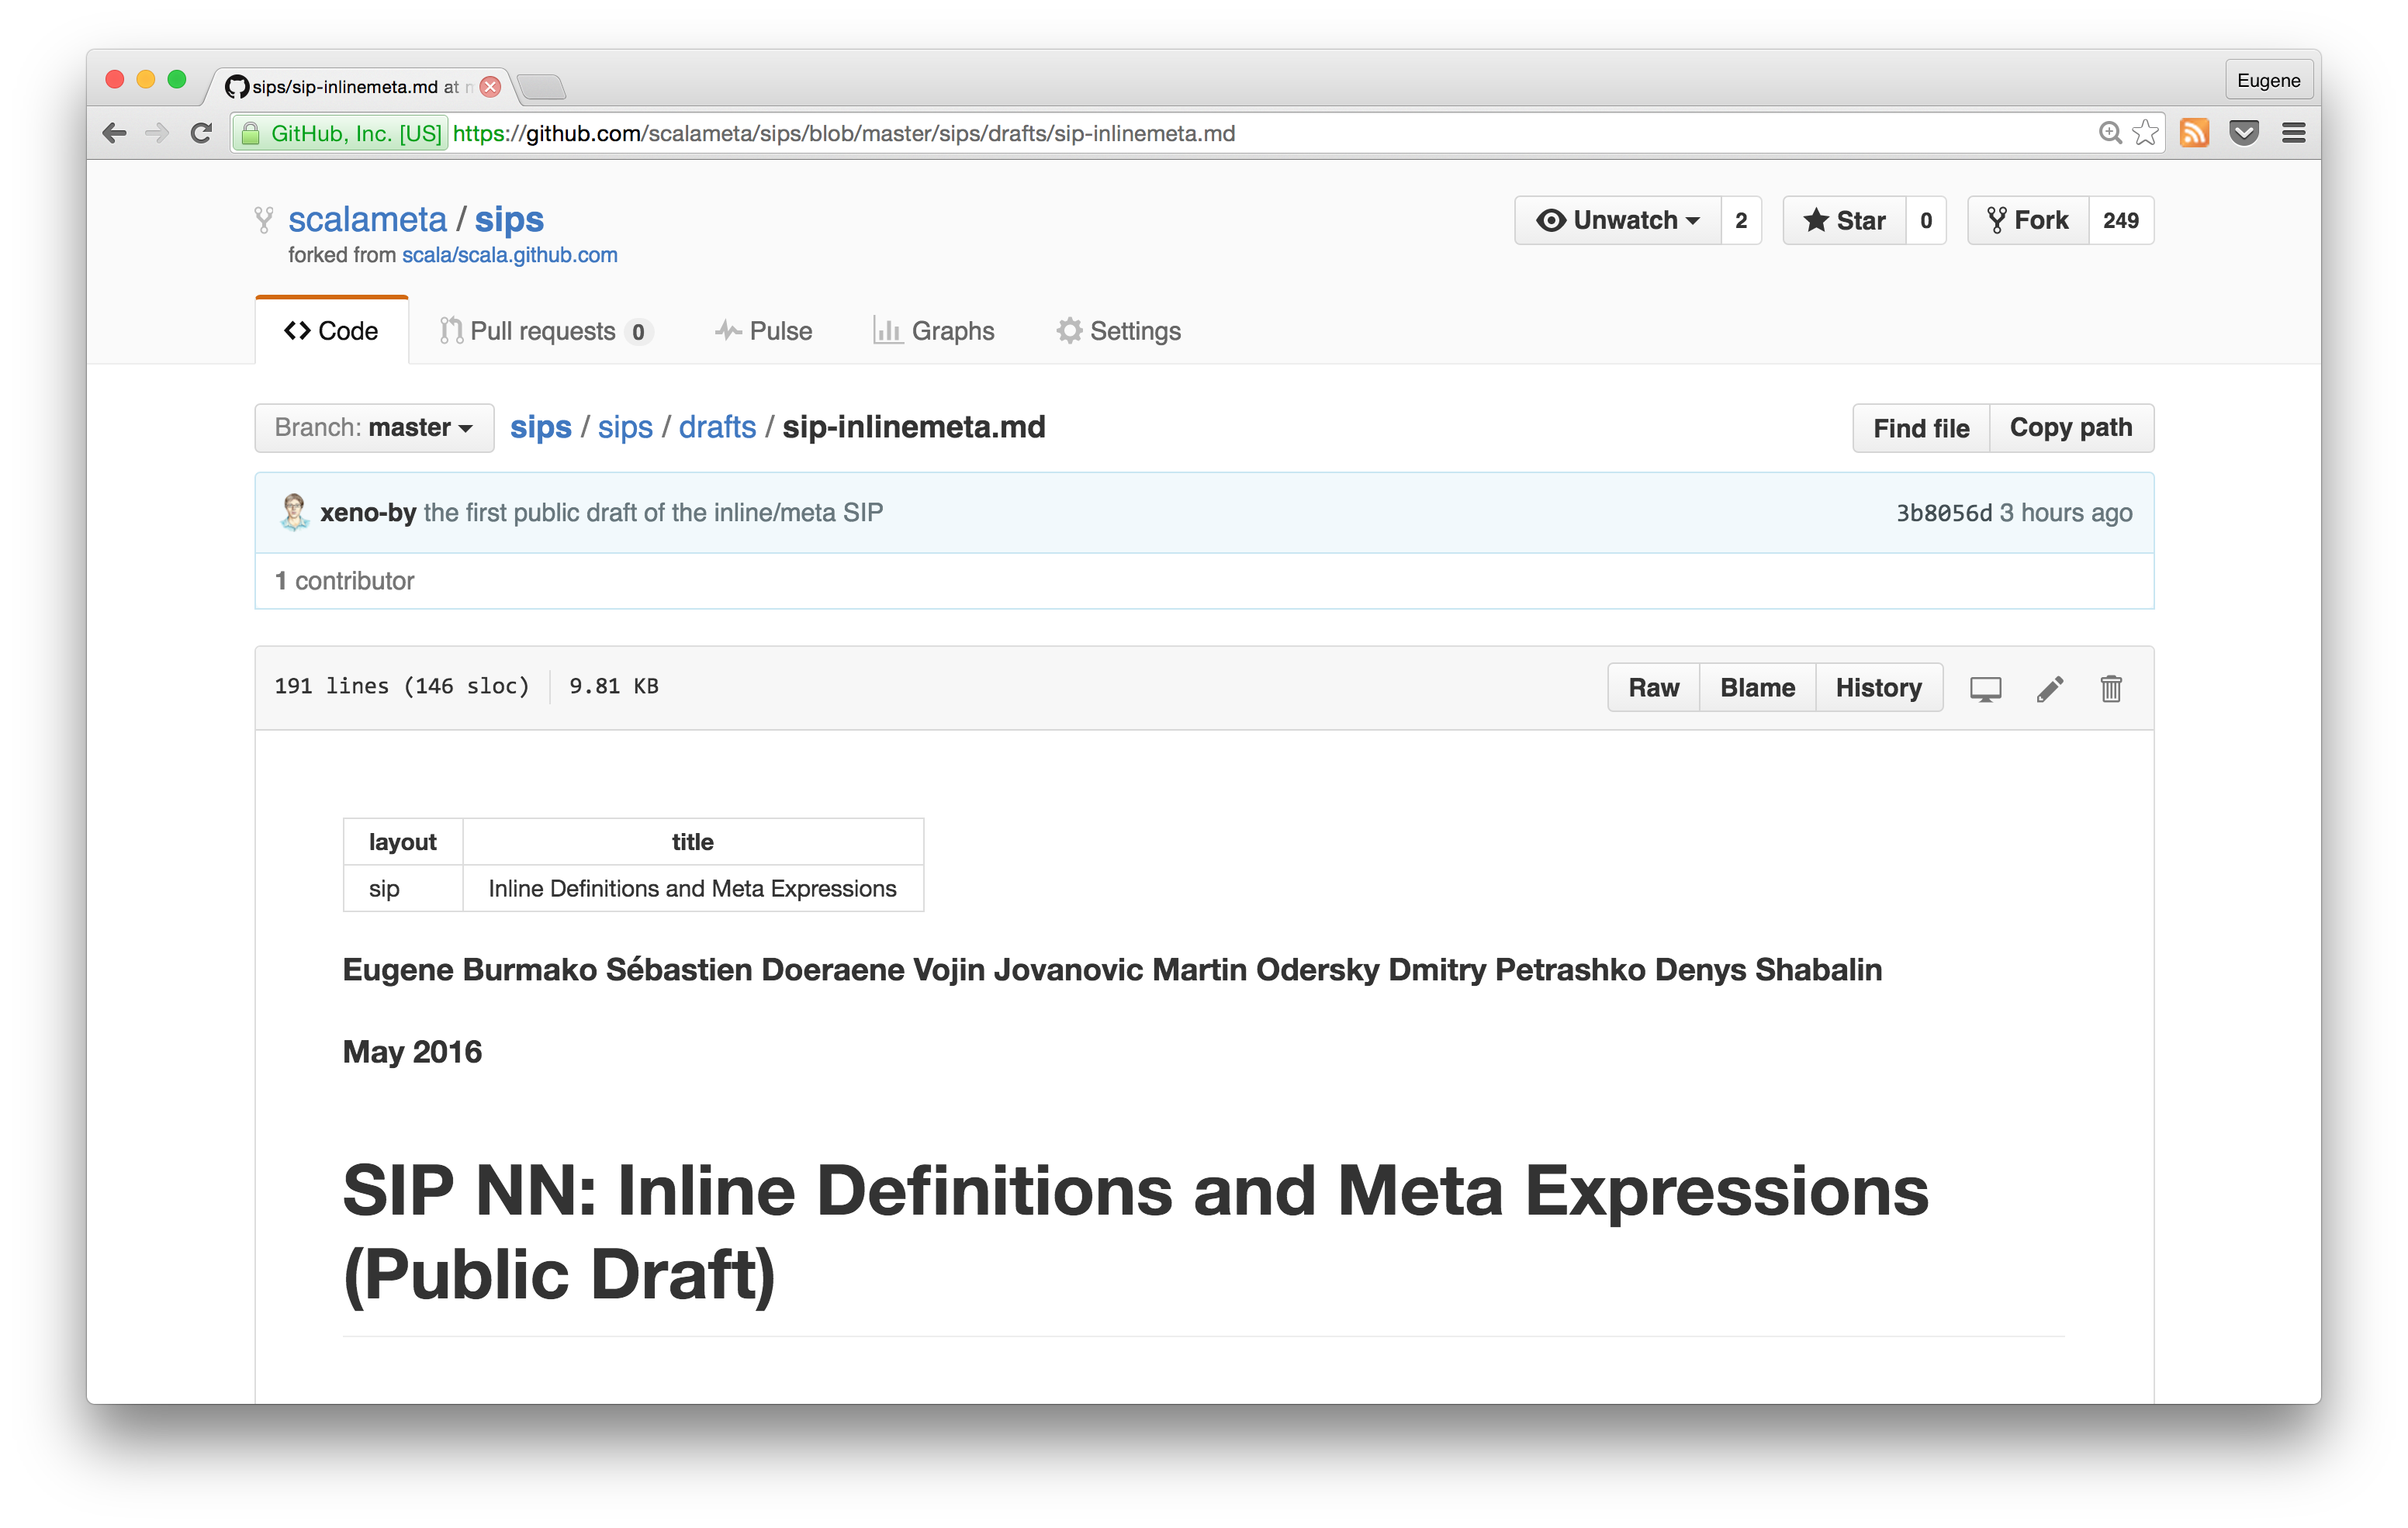
\includegraphics[height=7.5cm]{inlinemeta-sip.png}
\end{center}
\end{frame}

\begin{frame}{The new future for macros}
\begin{itemize}
\item \text{\color{blue}\href{https://github.com/scalameta/sips/blob/master/sips/drafts/sip-inlinemeta.md}{SIP NN: Inline Definitions and Meta Expressions}}
\item We got to the essence of macros and found two orthogonal concepts
\item \texttt{inline} for inlining and \texttt{meta} for metaprogramming
\end{itemize}
\end{frame}

\begin{frame}[fragile]{Old macros}
\begin{semiverbatim}
class Table[T](val query: Query[T]) \{
  def map[U](fn: T => U): Table[U] = macro Macros.map
\}

object Macros \{
  def map(c: Context)(fn: c.Tree): c.Tree = \{
    val subquery: c.Tree = translate(fn)
    q"new Table(Map(\$\{c.prefix\}, \$subquery))"
  \}
\}
\end{semiverbatim}
\end{frame}

\begin{frame}[fragile]{Old macros}
\begin{semiverbatim}
val users: Table[User] = ...
users.map(u => u.name)

                          \arrowdown

val users: Table[User] = ...
new Table(Map(users, Ref("name", classOf[String])))

\end{semiverbatim}

\begin{itemize}
\item When the user writes \texttt{Table.map}, \text{\color<2->{blue}{the compiler calls \texttt{Macros.map}}}
\item \texttt{Macros.map} expands in a domain-specific fashion
\item \text{\color<3->{red}{Compiler replaces the call to \texttt{Table.map} with the macro expansion}}
\end{itemize}
\end{frame}

\begin{frame}[fragile]{New macros}
\begin{semiverbatim}
class Table[T](val query: Query[T]) \{
  inline def map[U](fn: T => U): Table[U] = meta \{
    val subquery: c.Tree = translate(fn)
    q"new Table(Map(\$this, \$subquery))"
  \}
\}
\end{semiverbatim}
\end{frame}

\begin{frame}[fragile]{New macros}
\begin{semiverbatim}
val users: Table[User] = ...
users.map(u => u.name)

                          \arrowdown

val users: Table[User] = ...
\text{\color<2->{red}{meta\{ ...; q"new Table(Map(users, \$subquery))" \}}}

                          \arrowdown

val users: Table[User] = ...
\text{\color<3->{blue}{new Table(Map(users, Ref("name", classOf[String])))}}

\end{semiverbatim}

\begin{itemize}
\item When the user writes \texttt{Table.map}, \text{\color<2->{red}{the compiler inlines its rhs}}
\item \text{\color<3->{blue}{Compiler expands the \texttt{meta} block using scala.meta}}
\item The results of the meta expansion are inlined again
\end{itemize}
\end{frame}

\sectionframe{Part 4: Live demo}

\begin{frame}{Challenge accepted}
\vskip20pt
\begin{center}
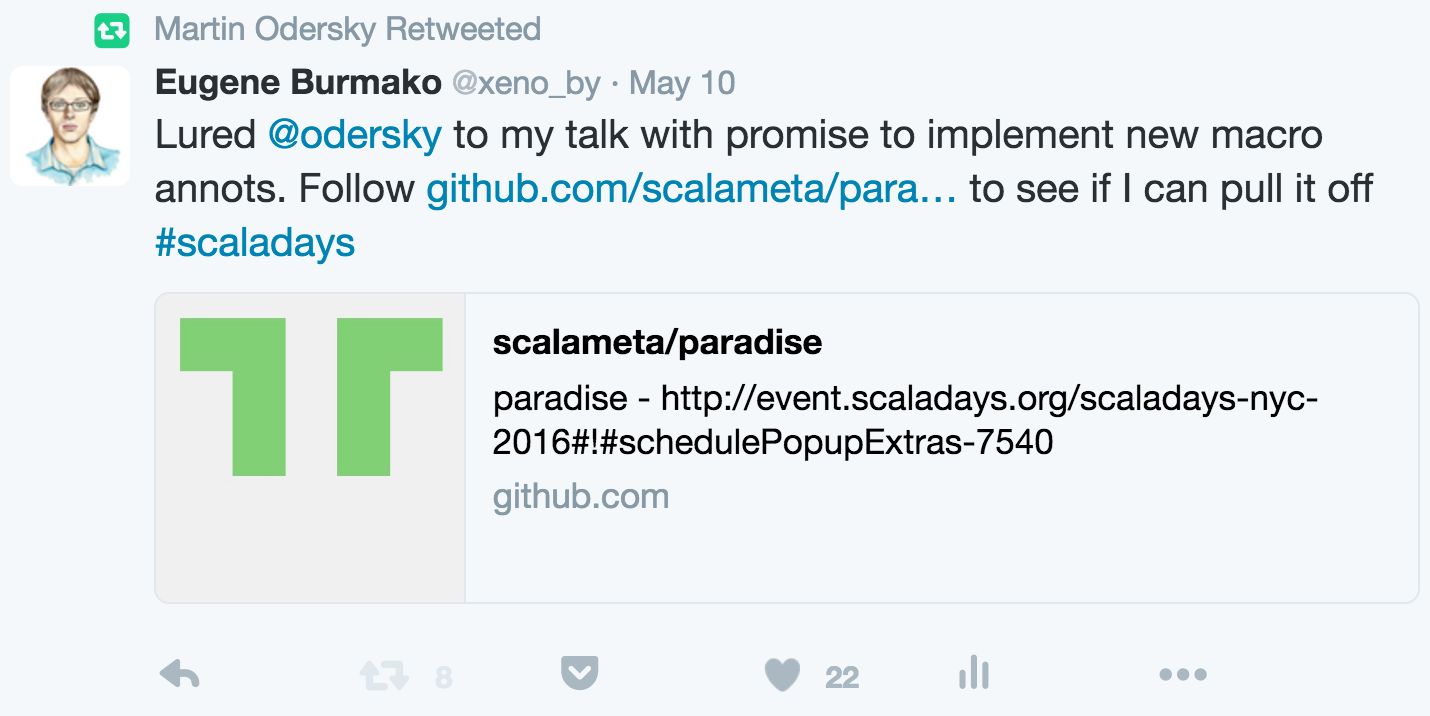
\includegraphics[height=6cm]{challenge-accepted.png}
\end{center}
\end{frame}

\begin{frame}{Mission accomplished}
\vskip20pt
\begin{center}
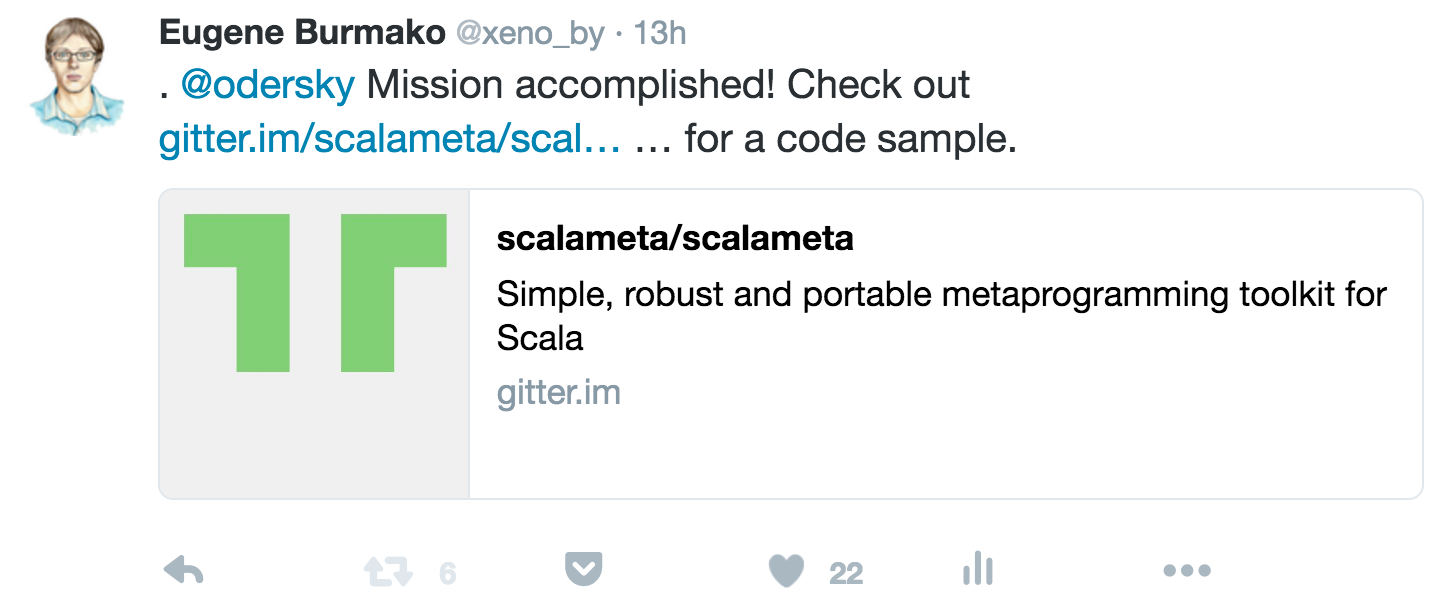
\includegraphics[height=5cm]{mission-accomplished.png}
\end{center}
\end{frame}

\begin{frame}{In the meanwhile, in the Dotty land}
\vskip20pt
\begin{center}
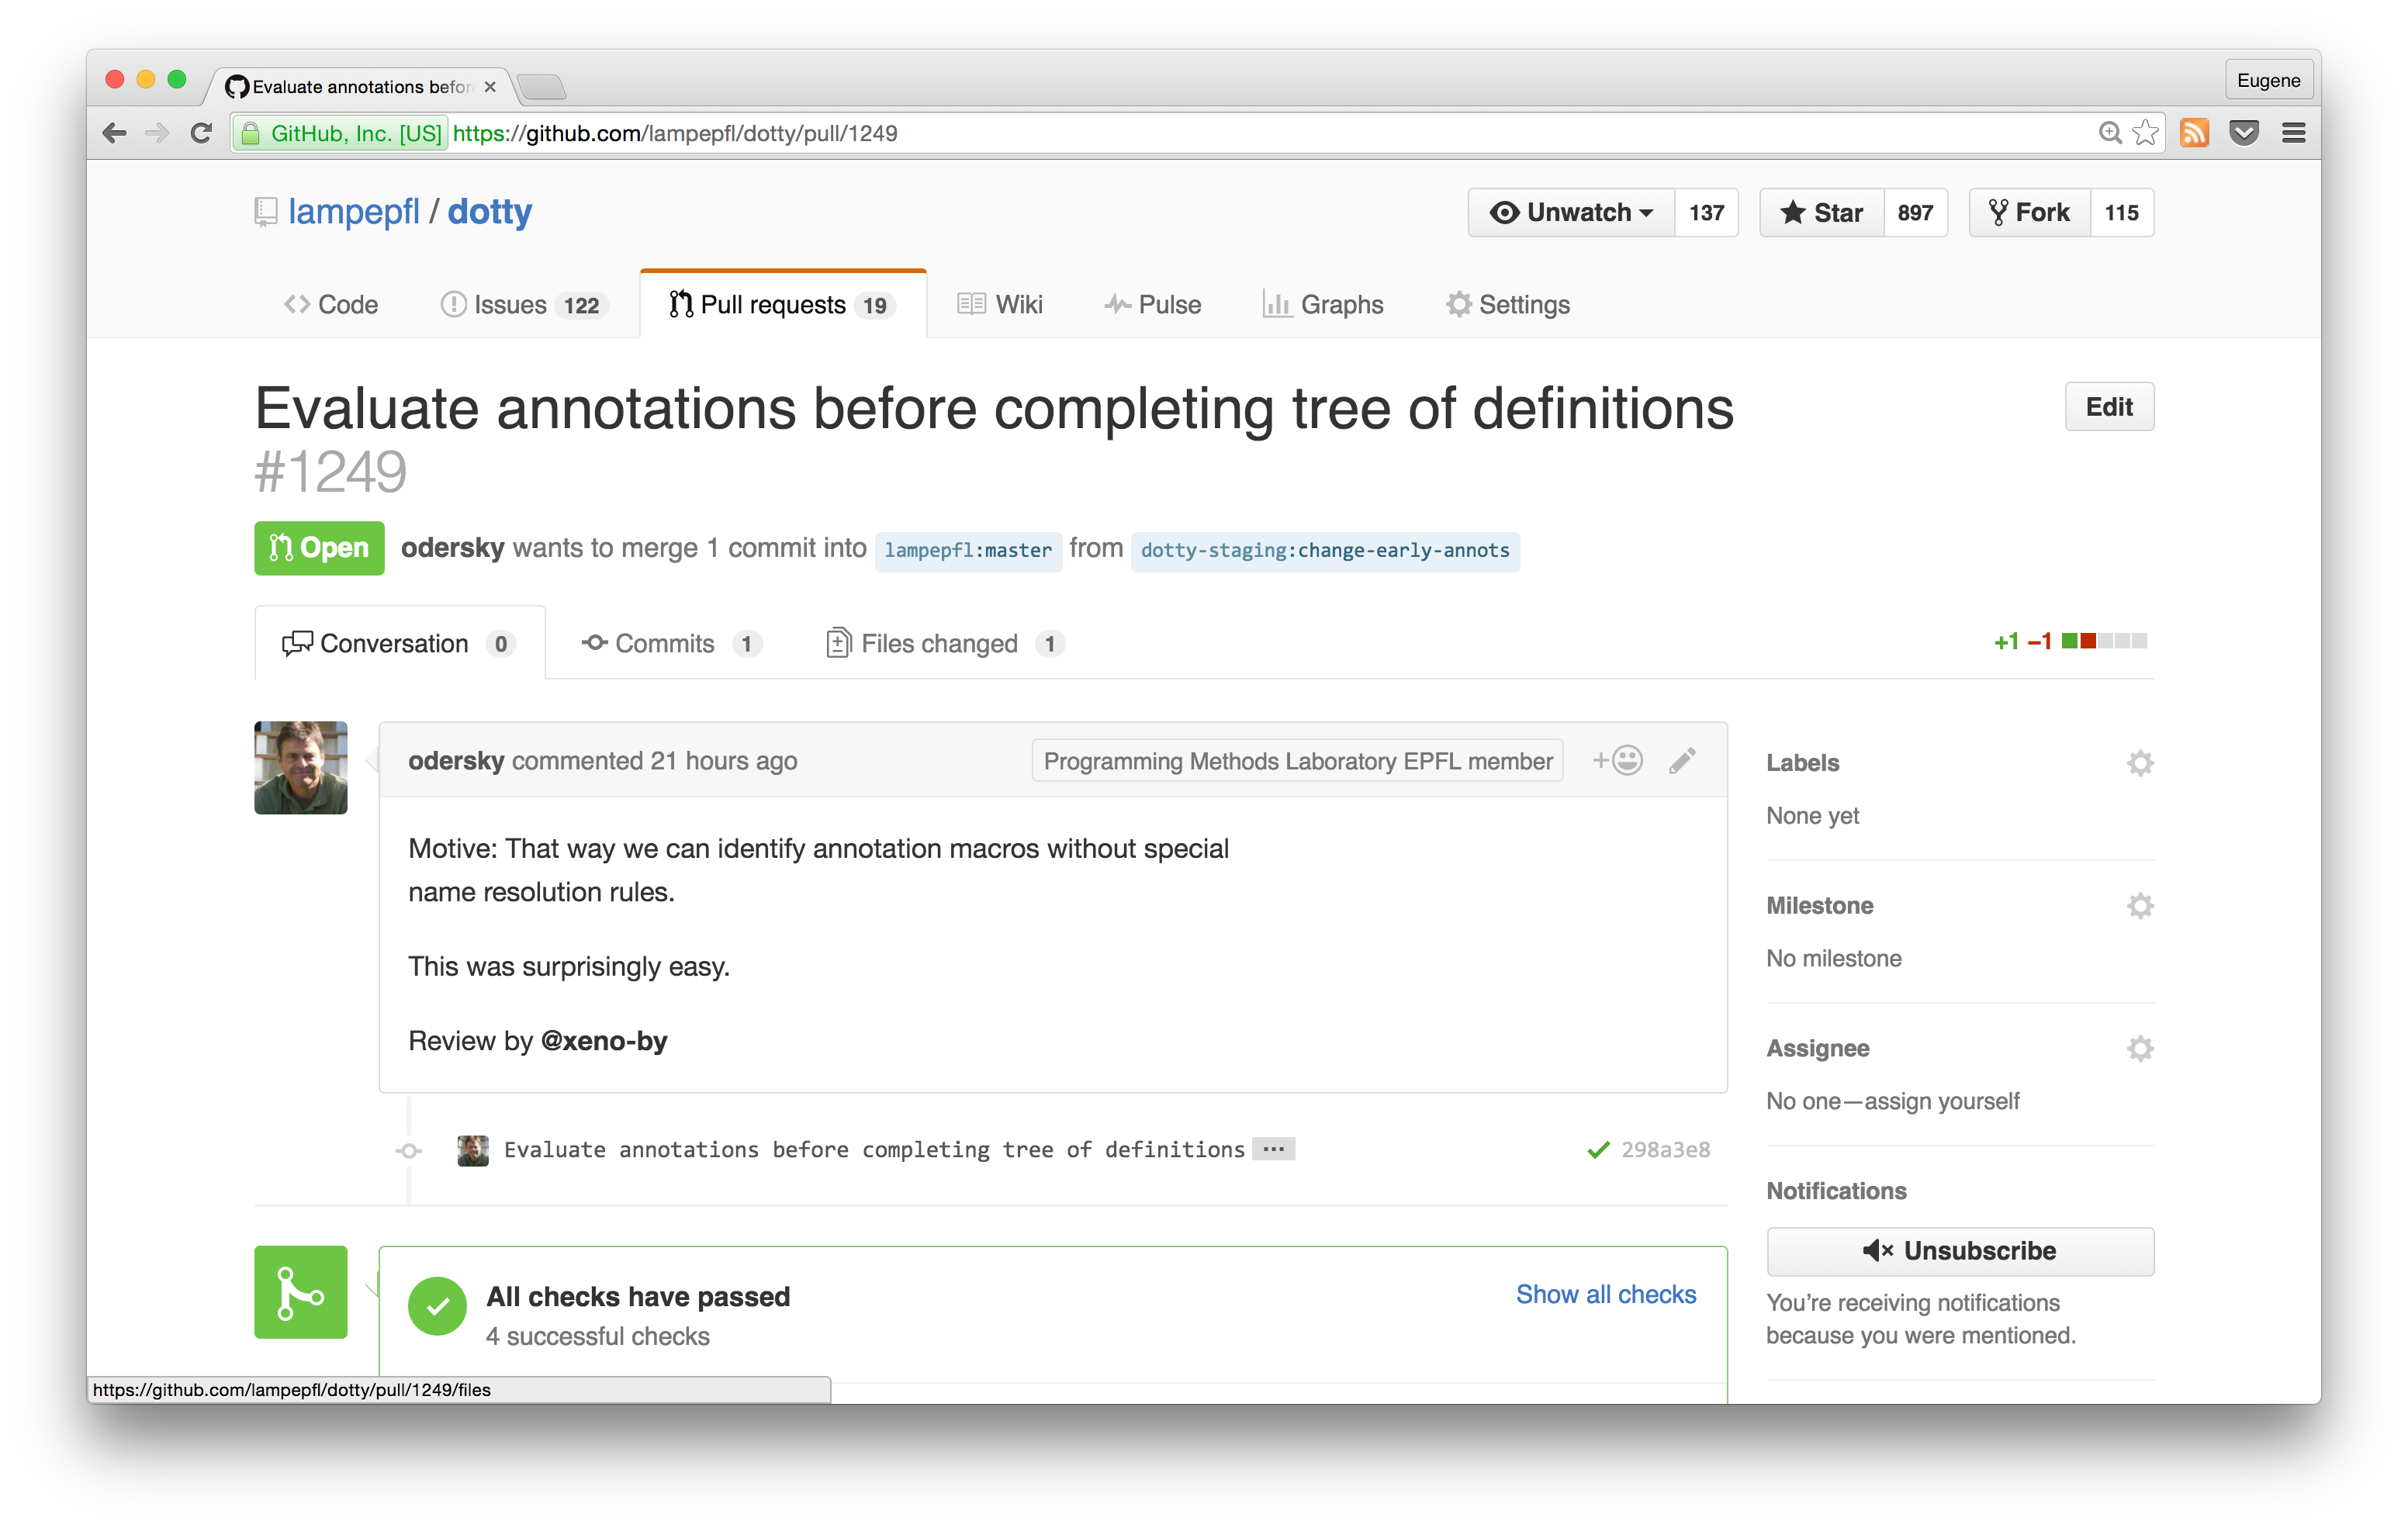
\includegraphics[height=7.5cm]{dotty-pr.png}
\end{center}
\end{frame}

\sectionframe{Part 5: The future}

\begin{frame}[c, fragile]{Codacy}
\begin{center}
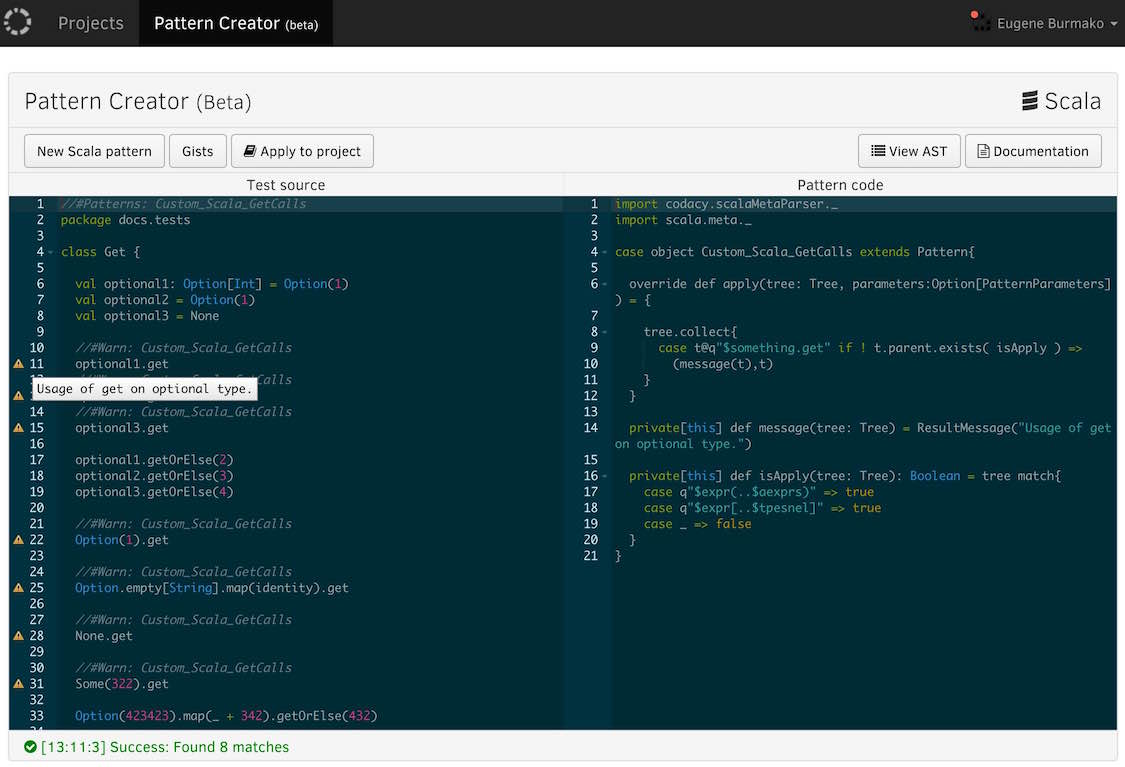
\includegraphics[height=7.5cm]{codacy.jpg}
\end{center}
\end{frame}

\begin{frame}[c, fragile]{scalafmt}
\vskip20pt
\begin{center}
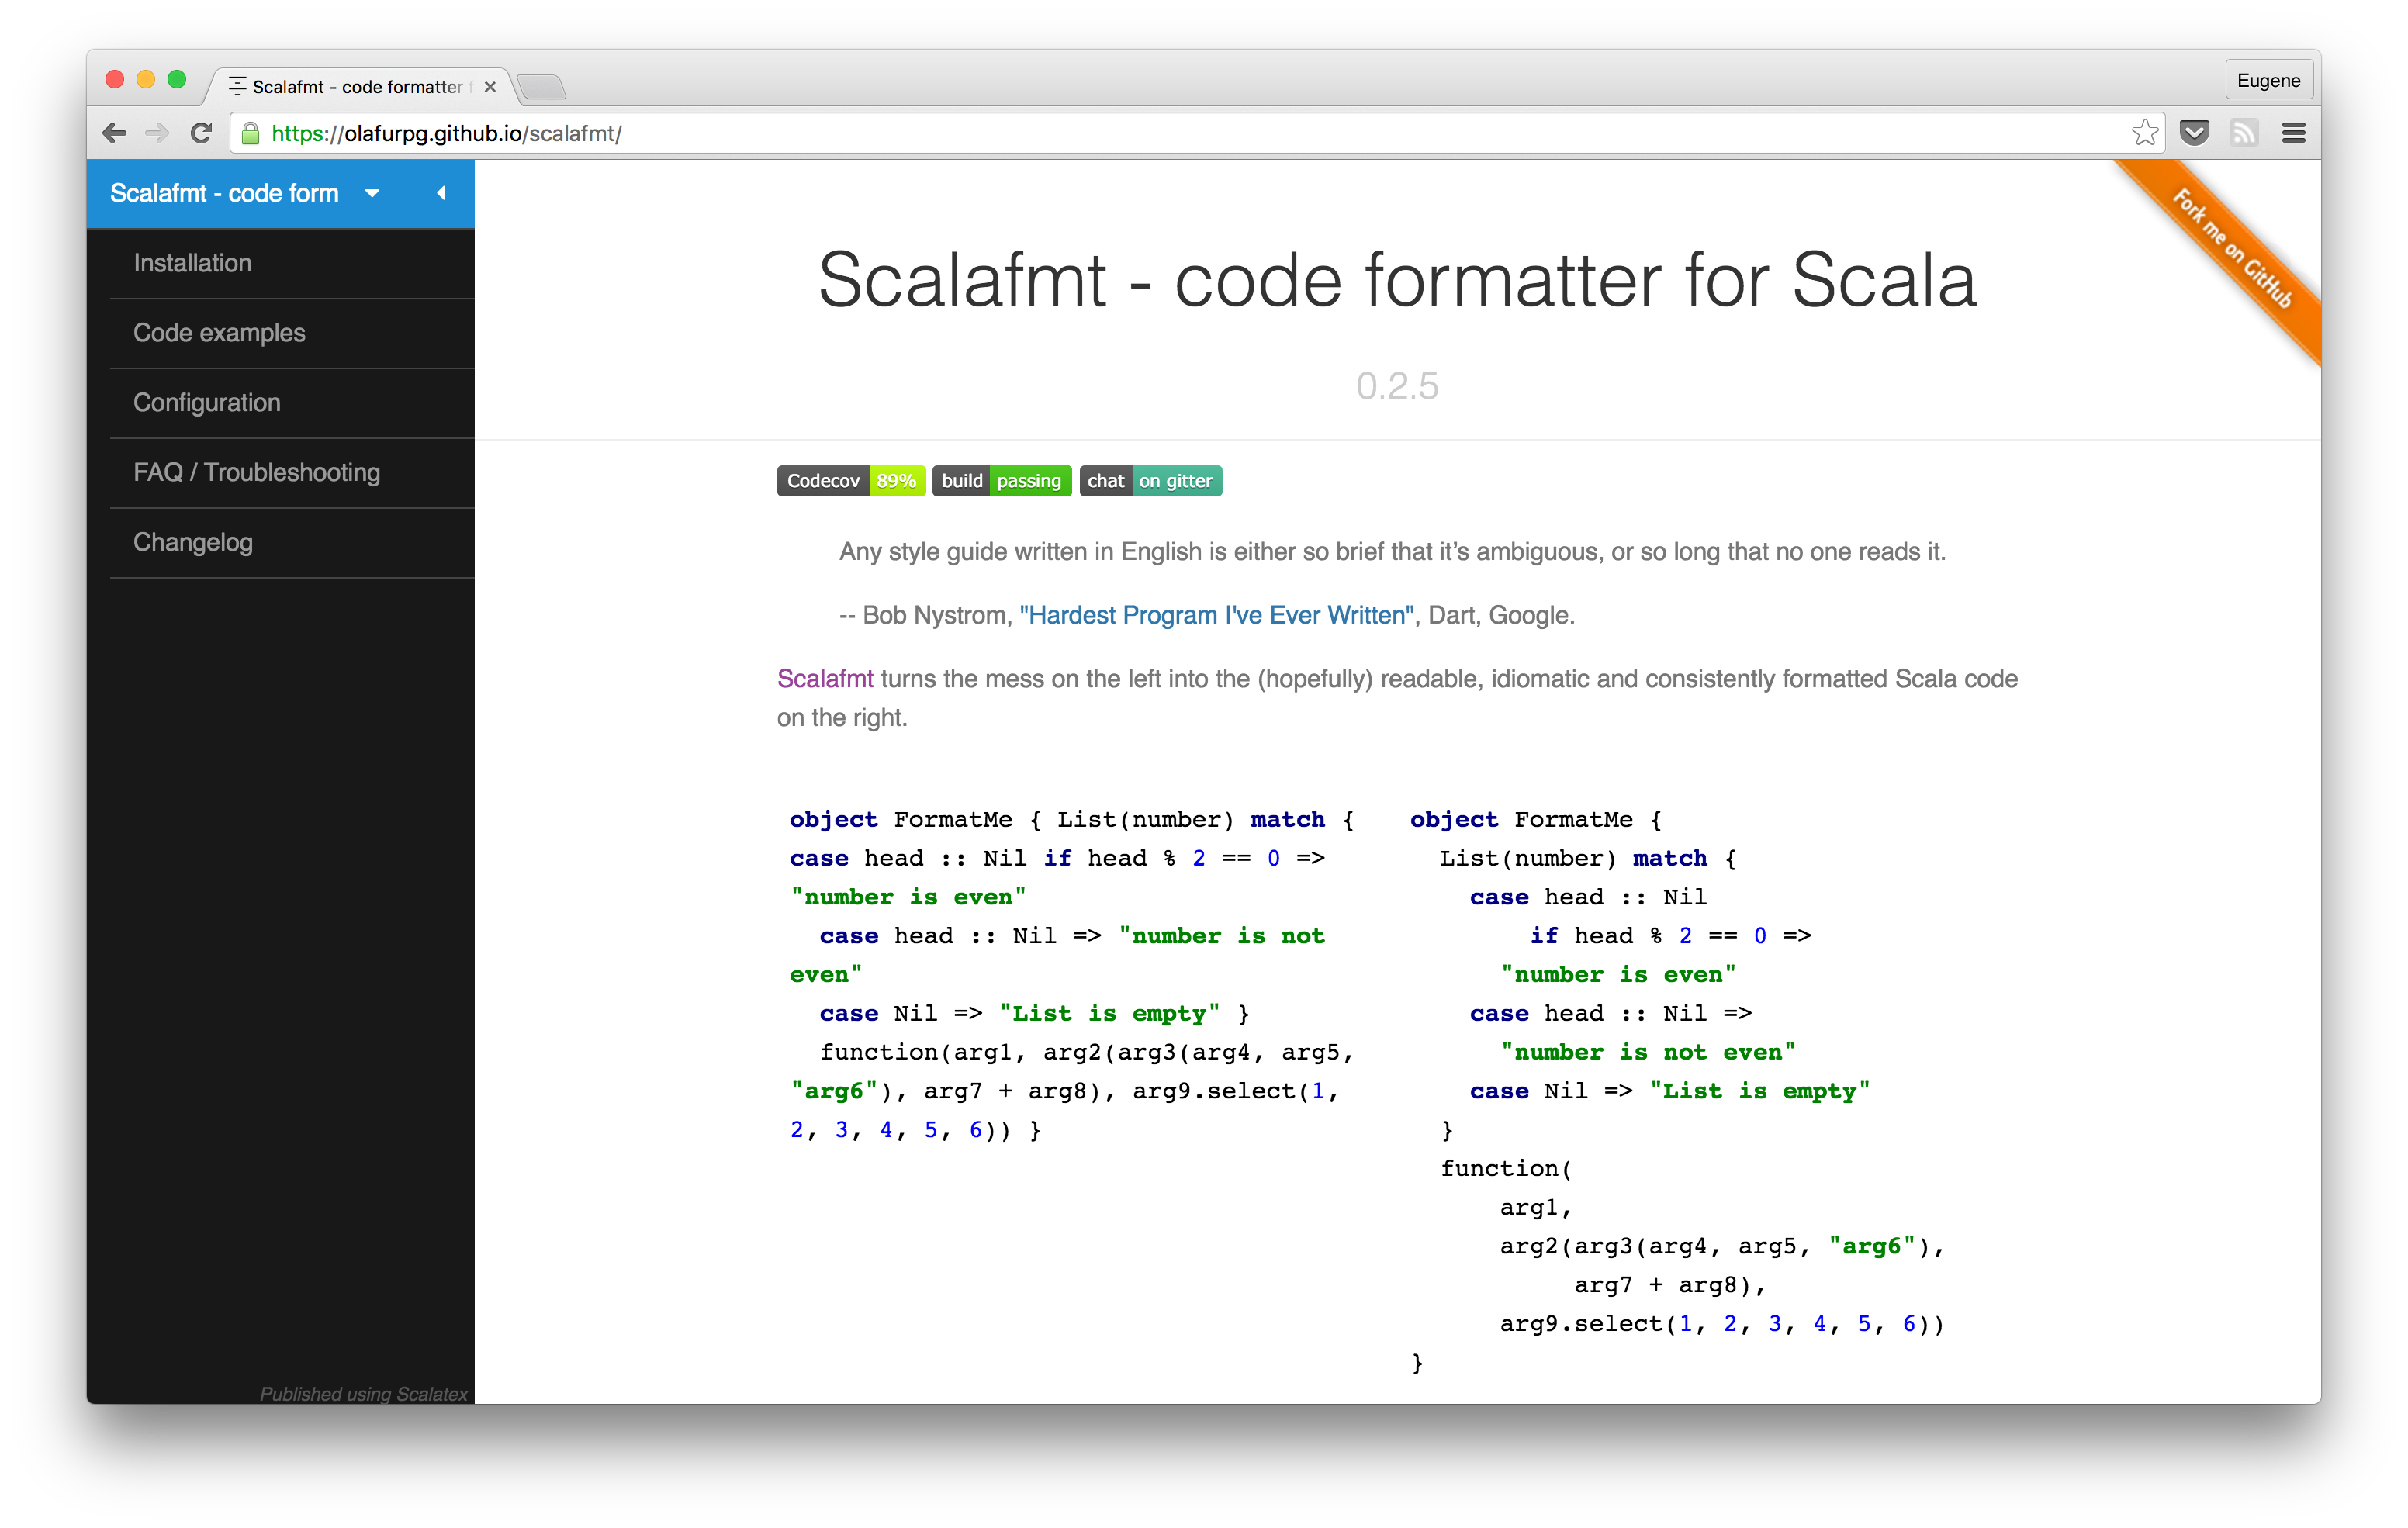
\includegraphics[height=7.5cm]{scalafmt.png}
\end{center}
\end{frame}

\begin{frame}[fragile]{Inline macros}
\begin{semiverbatim}
import scala.meta._

object main \{
  inline def apply()(defn: Any) = meta \{
    val q"object \$name { ..\$stats }" = defn
    val main = q"""
      def main(args: Array[String]): Unit = \{ ..\$stats \}
    """
    q"object \$name \{ \$main \}"
  \}
\}

@main object Test \{
  println("hello world")
\}
\end{semiverbatim}
\end{frame}

\begin{frame}[fragile]{Dotty linker}
\begin{semiverbatim}
import dotty.linker._

@rewrites
object Rewrites \{
  def metaRule[T](x: List[T]) =
    Rewrite(from = x.toString,
              to = meta \{ /* entry point to scala.meta */ \})
\}
\end{semiverbatim}
\end{frame}

\begin{frame}[c, fragile]{}
\begin{center}
% https://twitter.com/phdcomics/status/337323601747406849
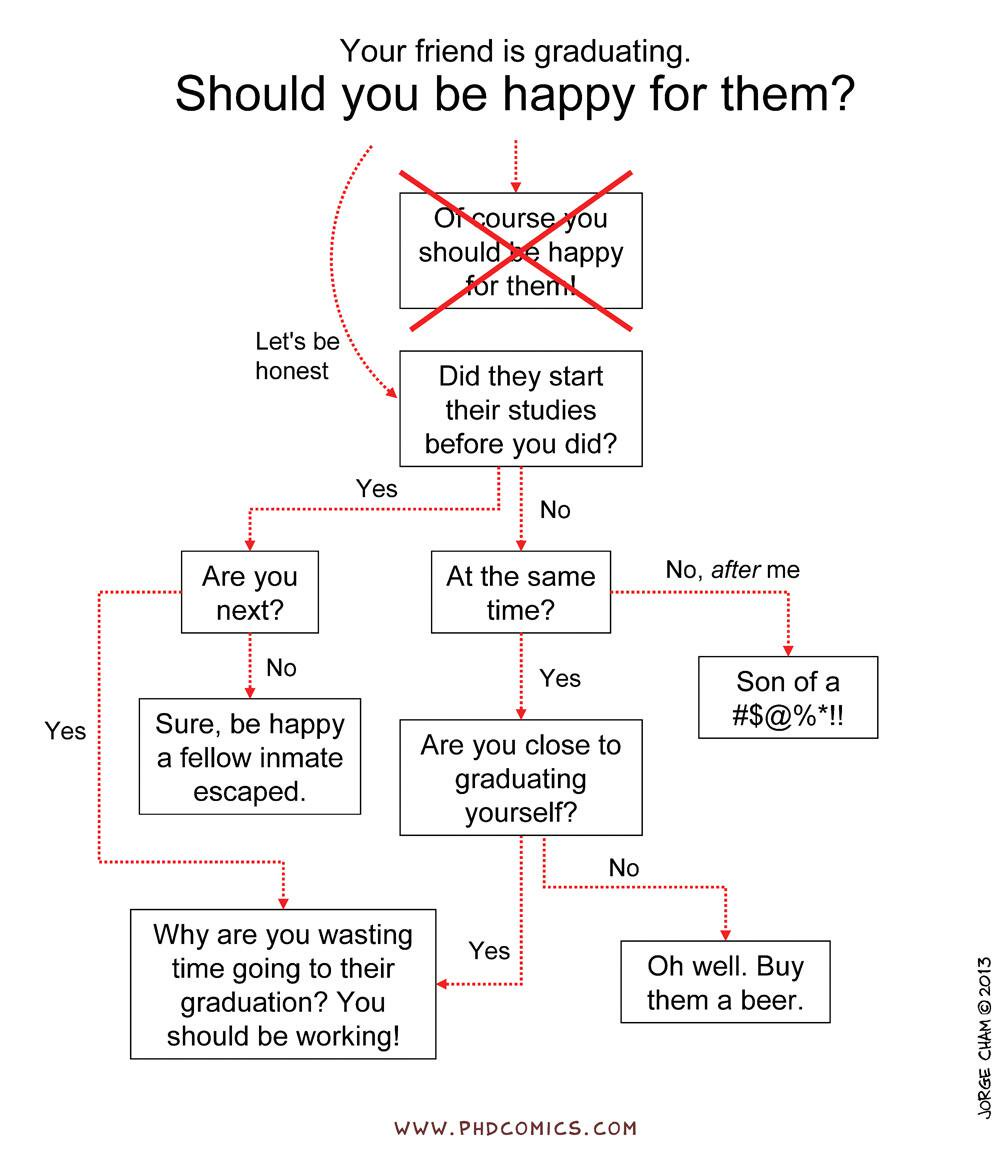
\includegraphics[height=7.5cm]{YourFriendIsGraduating.jpg}\\
\end{center}
\end{frame}

\begin{frame}{The road ahead}
\vskip20pt
\begin{center}

\includegraphics[height=4cm]{twitter.png}
\end{center}
\end{frame}

\sectionframe{Wrapping up}

\begin{frame}{Summary}
\begin{itemize}
\item We've just released our first beta version
\item The project is officially endorsed and funded
\item Current users: Codacy, scalafmt
\item Future users: new macros, Dotty linker
\item Try it out!
\end{itemize}
\end{frame}

\end{document}
